% Options for packages loaded elsewhere
\PassOptionsToPackage{unicode}{hyperref}
\PassOptionsToPackage{hyphens}{url}
%
\documentclass[
  12pt,
]{article}
\usepackage{amsmath,amssymb}
\usepackage{iftex}
\ifPDFTeX
  \usepackage[T1]{fontenc}
  \usepackage[utf8]{inputenc}
  \usepackage{textcomp} % provide euro and other symbols
\else % if luatex or xetex
  \usepackage{unicode-math} % this also loads fontspec
  \defaultfontfeatures{Scale=MatchLowercase}
  \defaultfontfeatures[\rmfamily]{Ligatures=TeX,Scale=1}
\fi
\usepackage{lmodern}
\ifPDFTeX\else
  % xetex/luatex font selection
\fi
% Use upquote if available, for straight quotes in verbatim environments
\IfFileExists{upquote.sty}{\usepackage{upquote}}{}
\IfFileExists{microtype.sty}{% use microtype if available
  \usepackage[]{microtype}
  \UseMicrotypeSet[protrusion]{basicmath} % disable protrusion for tt fonts
}{}
\makeatletter
\@ifundefined{KOMAClassName}{% if non-KOMA class
  \IfFileExists{parskip.sty}{%
    \usepackage{parskip}
  }{% else
    \setlength{\parindent}{0pt}
    \setlength{\parskip}{6pt plus 2pt minus 1pt}}
}{% if KOMA class
  \KOMAoptions{parskip=half}}
\makeatother
\usepackage{xcolor}
\usepackage[margin=1in]{geometry}
\usepackage{graphicx}
\makeatletter
\def\maxwidth{\ifdim\Gin@nat@width>\linewidth\linewidth\else\Gin@nat@width\fi}
\def\maxheight{\ifdim\Gin@nat@height>\textheight\textheight\else\Gin@nat@height\fi}
\makeatother
% Scale images if necessary, so that they will not overflow the page
% margins by default, and it is still possible to overwrite the defaults
% using explicit options in \includegraphics[width, height, ...]{}
\setkeys{Gin}{width=\maxwidth,height=\maxheight,keepaspectratio}
% Set default figure placement to htbp
\makeatletter
\def\fps@figure{htbp}
\makeatother
\setlength{\emergencystretch}{3em} % prevent overfull lines
\providecommand{\tightlist}{%
  \setlength{\itemsep}{0pt}\setlength{\parskip}{0pt}}
\setcounter{secnumdepth}{-\maxdimen} % remove section numbering
\usepackage{setspace}\doublespacing
\ifLuaTeX
  \usepackage{selnolig}  % disable illegal ligatures
\fi
\IfFileExists{bookmark.sty}{\usepackage{bookmark}}{\usepackage{hyperref}}
\IfFileExists{xurl.sty}{\usepackage{xurl}}{} % add URL line breaks if available
\urlstyle{same}
\hypersetup{
  pdftitle={Multiple Linear Regression Modeling of Test Scores using Socioeconomical Factors},
  pdfauthor={Miao Fu(mf3593)},
  hidelinks,
  pdfcreator={LaTeX via pandoc}}

\title{Multiple Linear Regression Modeling of Test Scores using
Socioeconomical Factors}
\author{Miao Fu(mf3593)}
\date{}

\begin{document}
\maketitle

\hypertarget{introduction}{%
\section{Introduction}\label{introduction}}

Education is an essential component of contemporary society, and the
assessment of student performance through test scores is commonly seen.
This research project focuses on studying the complex relationship
between various socioeconomic factors and the test scores of public
school students. Key variables, including ethnic group, parents' marital
status, and weekly study hours, are considered as potential predictive
variables of test score outcomes. Through statistical modeling, we aim
to identify significant contributing factors and construct predictive
models, providing a thorough understanding of the dynamics between
socioeconomic factors and test performance.

The chosen 11 covariates represent a spectrum of influences within
students' socioenvironmental contexts and are presumed to be potentially
relevant to one's academic performance. By combining all these factors
into predictive models, our research aims to select out the variables
that significantly shape test performance and recommend a final optimal
model for each of three test scores(maths, writing, reading).
Additionally, model comparisons will be conducted to evaluate the
associations between covariates and test scores in a detailed and
comprehensive way. This study contributes to the broader understanding
of educational equity and may inform potential interventions to create a
better education environment at public schools.

\hypertarget{methods}{%
\section{Methods}\label{methods}}

The dataset used contained 587 observations and 14 variables.

Data exploration was first done by obtaining descriptive summary
statistics for all variables. Percentage and count of each category was
obtained for categorical variables(Figure 1). Mean, median, standard
deviation, minimum, maximum, q1 and q3 were obtained for numeric
variables(Figure 2). The normality of distribution of outcome variables
were investigated by plotting the data on histogram, boxplot, and QQ
plots. Normality of distribution of all variables were studied by
histogram(Figure 3). From the distribution bar graphs, it was decided
that no transformation is needed for any predictor variables.
Admittedly, the distributions might not be good references for
transformation because the variables are all categorical. Since the
distribution of the three scores showed slightly left-tailed, three
types of transformations were tested: 1) Natural logarithm 2) Square
Root 3) Inverse. The resulting plots are plotted in histograms(Figure
4). There is no apparent improvement on the distribution of the outcome
through the three transformations. Thus, the original outcome data were
chosen to be used in following statistical modeling steps.

By plotting our the pairwise correlation between variables, there is
apparent linearity among the three scores(Figure 5). Other correlation
coefficients are relatively small, indicating weak linear relationship
between the variables.\\

\begin{figure}
  \centering
  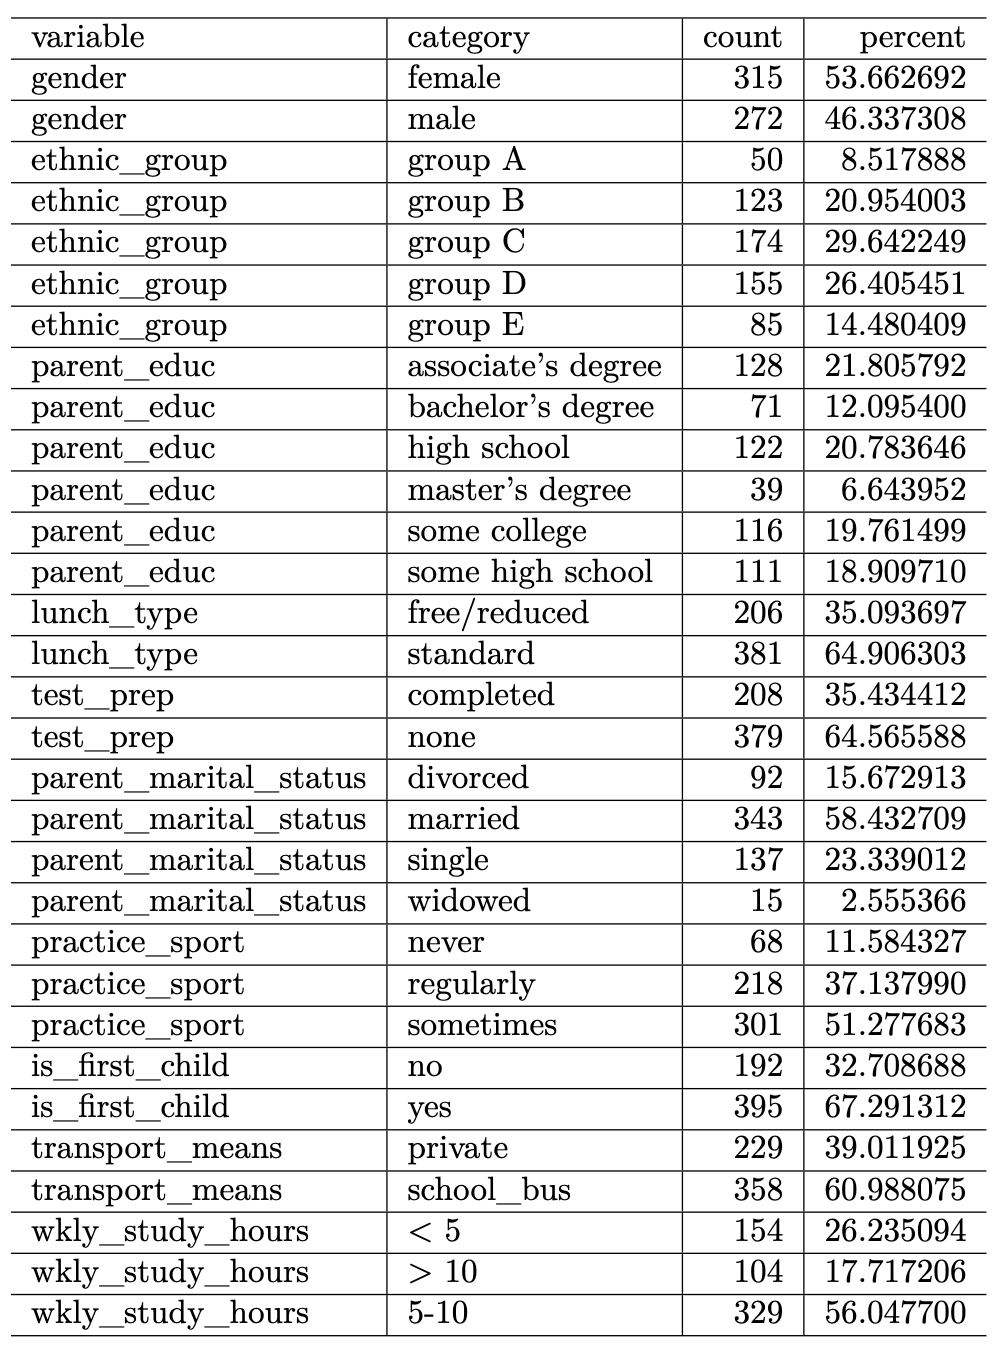
\includegraphics[width=0.5\textwidth]{table1.png}
  \caption{Summary Statistics of Categorical Variables}
\end{figure}

\begin{figure}
  \centering
  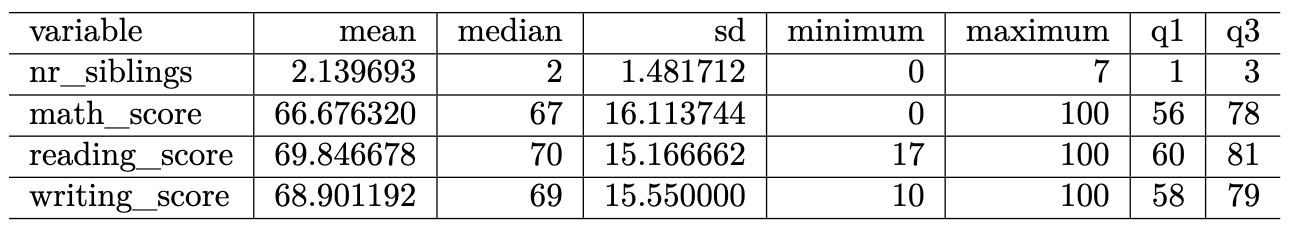
\includegraphics[width=0.5\textwidth]{table2.png}
  \caption{Summary Statistics of Numeric Variables}
\end{figure}

\begin{figure}
  \centering
  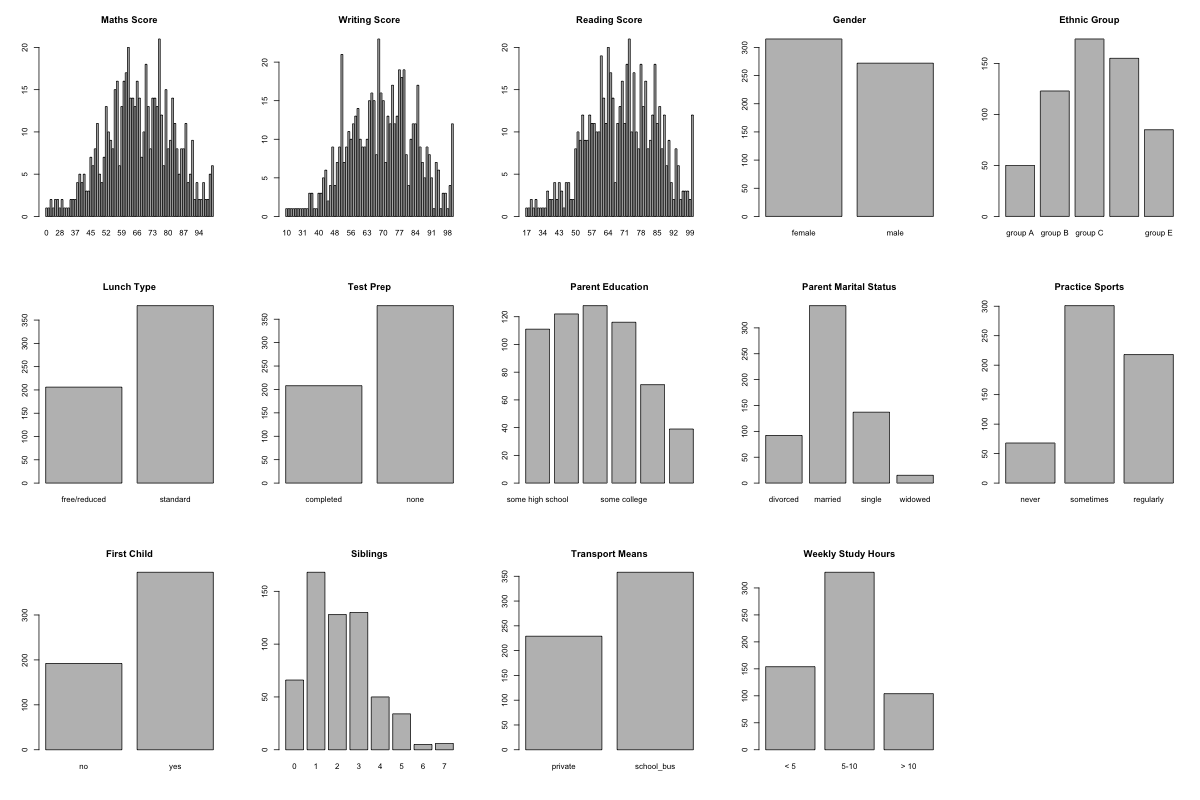
\includegraphics[width=0.5\textwidth]{normality_check.png}
  \caption{Histogram Distribution of All Variables}
\end{figure}

\begin{figure}
  \centering
  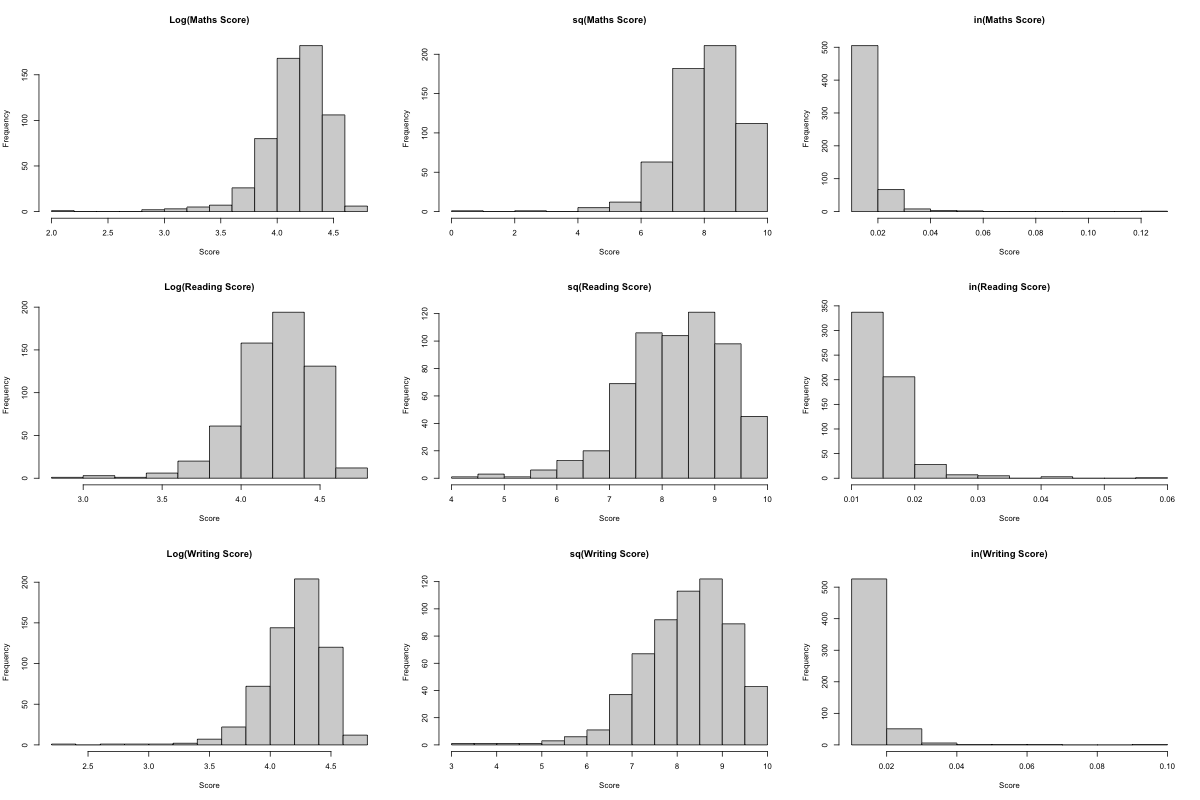
\includegraphics[width=0.5\textwidth]{transformation_check.png}
  \caption{Log, sqrt, and inverse transformation of the outcome variables}
\end{figure}

\begin{figure}
  \centering
  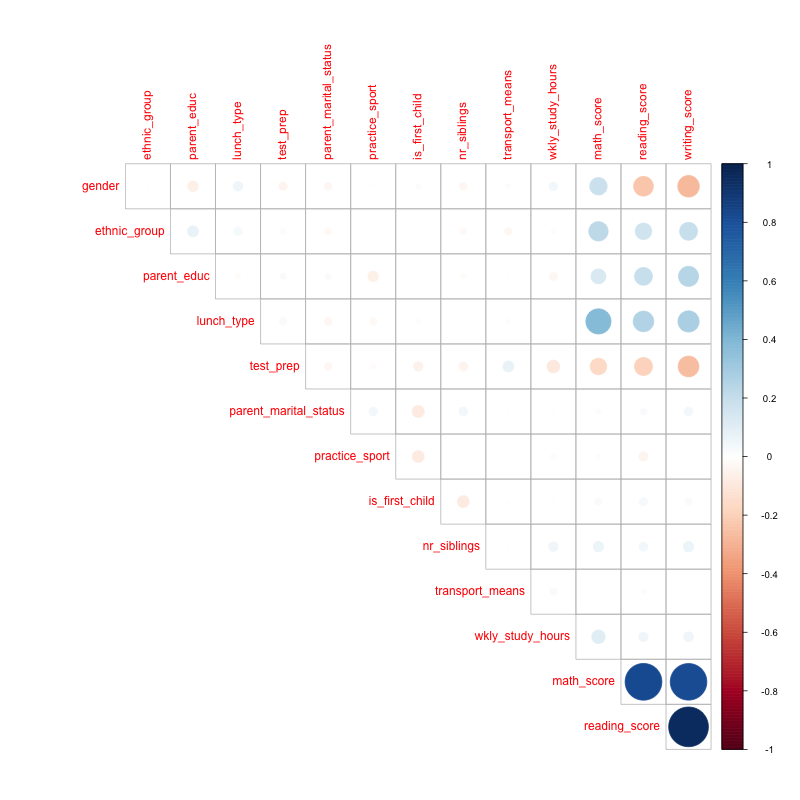
\includegraphics[width=0.5\textwidth]{correlation_plot.png}
  \caption{Correlation plot between variables}
\end{figure}

\newpage

\hypertarget{discussion}{%
\section{Discussion}\label{discussion}}

To study whether it is possible to leverage one or two scores to improve
the model of scores, a new MLR for each score was created by adding the
rest two scores as predictors alongside with the original covariates
obtianed through previous model selection. MSE was calculated for each
model and compared (Figure 6). We can see that the MSE all significantly
decreased after adding other scores to fit one score's model, indicating
that leveraging other scores to enhance one score's model is possible
and successful .

\begin{figure}
  \centering
  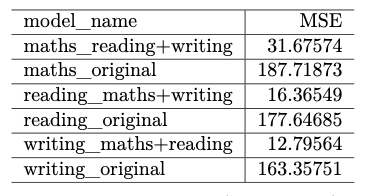
\includegraphics[width=0.5\textwidth]{table3.png}
  \caption{MSE of models after addition of other scores}
\end{figure}

\hypertarget{contribution-summary}{%
\section{Contribution Summary}\label{contribution-summary}}

All four team members contributed equally to the project. Miao conducted
data exploration of the dataset, evaluation of leveraging scores to
enhance selected best model, and drafting introduction as well as parts
of the methods and disucssion sections.

\end{document}
